\documentclass[10pt]{article}
\usepackage[utf8]{inputenc}
\usepackage[margin=0in,paperwidth=12in,paperheight=4in]{geometry}
\usepackage{tikz}
\usepackage{xcolor}
\usepackage{amsmath,amssymb}
\usetikzlibrary{shapes.geometric, arrows.meta, positioning, calc, backgrounds}
\pagestyle{empty}

\definecolor{bgdark}{HTML}{0F172A}
\definecolor{cardbg}{HTML}{1E293B}
\definecolor{bordercol}{HTML}{334155}
\definecolor{accentblue}{HTML}{38BDF8}
\definecolor{accentgreen}{HTML}{10B981}
\definecolor{accentorange}{HTML}{F59E0B}
\definecolor{accentpurple}{HTML}{A855F7}
\definecolor{accentred}{HTML}{EF4444}
\definecolor{accentcyan}{HTML}{06B6D4}
\definecolor{textwhite}{HTML}{F8FAFC}
\definecolor{textmuted}{HTML}{94A3B8}

\begin{document}
\noindent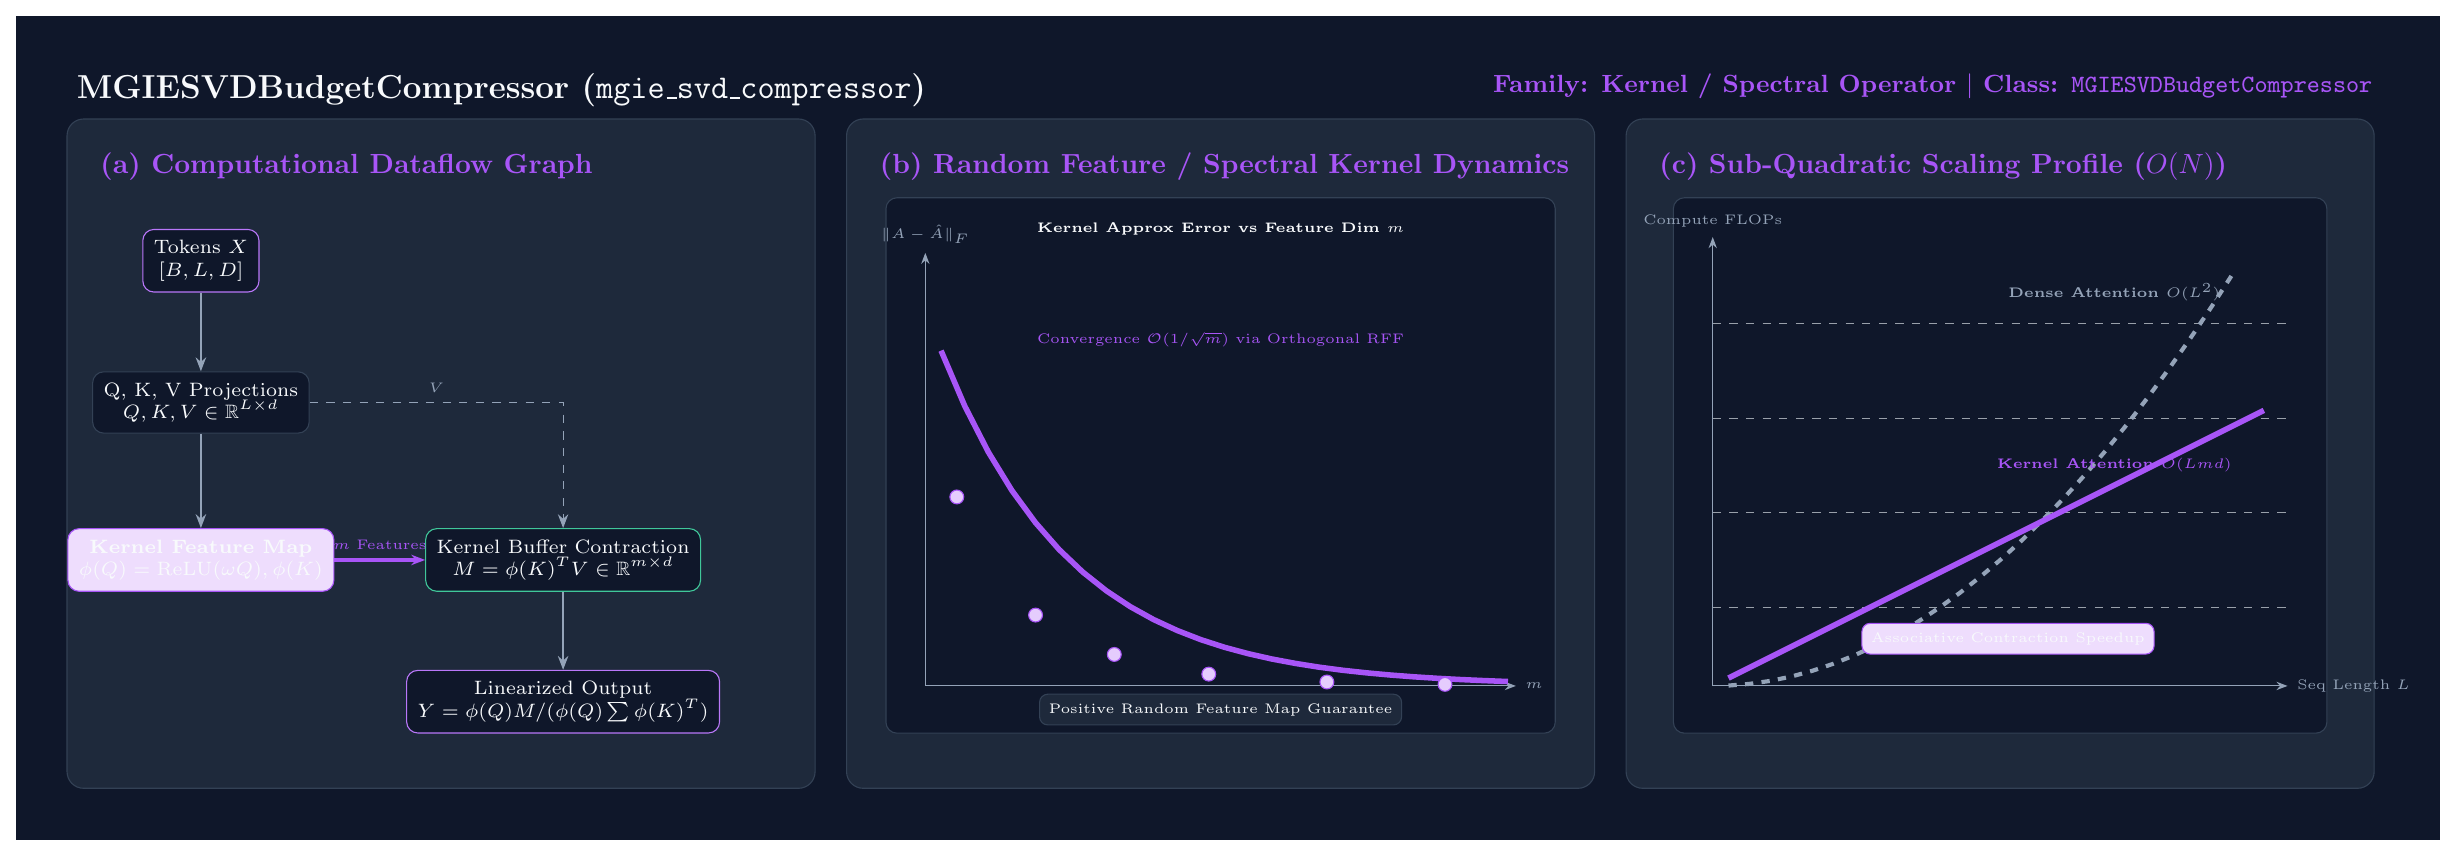
\begin{tikzpicture}[
    background rectangle/.style={fill=bgdark}, show background rectangle,
    scale=1.0, every node/.style={transform shape}
]

\clip (0,0) rectangle (30.48, 10.16);

% Title Header
\node[anchor=north west, text=textwhite, font=\large\bfseries] at (0.5, 9.7) {MGIESVDBudgetCompressor (\texttt{mgie\_svd\_compressor})};
\node[anchor=north east, text=accentpurple, font=\small\bfseries] at (29.9, 9.7) {Family: Kernel / Spectral Operator $\mid$ Class: \texttt{MGIESVDBudgetCompressor}};

% Panel A: Computational Architecture
\draw[fill=cardbg, draw=bordercol, rounded corners=6pt] (0.5, 0.5) rectangle (10.0, 9.0);
\node[anchor=north west, text=accentpurple, font=\bfseries\normalsize] at (0.8, 8.7) {(a) Computational Dataflow Graph};

\node[draw=accentpurple!80, fill=bgdark, rounded corners=4pt, text=textwhite, font=\scriptsize, align=center, inner sep=4pt] (inp) at (2.2, 7.2) {Tokens $X$\\$[B, L, D]$};
\node[draw=bordercol, fill=bgdark, rounded corners=4pt, text=textwhite, font=\scriptsize, align=center, inner sep=4pt] (proj) at (2.2, 5.4) {Q, K, V Projections\\$Q, K, V \in \mathbb{R}^{L \times d}$};
\node[draw=accentpurple, fill=accentpurple!20, rounded corners=4pt, text=textwhite, font=\scriptsize\bfseries, align=center, inner sep=4pt] (core) at (2.2, 3.4) {Kernel Feature Map\\$\phi(Q) = \mathrm{ReLU}(\omega Q), \phi(K)$};
\node[draw=accentgreen!80, fill=bgdark, rounded corners=4pt, text=textwhite, font=\scriptsize, align=center, inner sep=4pt] (gate) at (6.8, 3.4) {Kernel Buffer Contraction\\$M = \phi(K)^T V \in \mathbb{R}^{m \times d}$};
\node[draw=accentpurple!80, fill=bgdark, rounded corners=4pt, text=textwhite, font=\scriptsize, align=center, inner sep=4pt] (outp) at (6.8, 1.6) {Linearized Output\\$Y = \phi(Q) M / (\phi(Q) \sum \phi(K)^T)$};

        \draw[-{Stealth[length=5pt]}, textmuted, line width=1pt] (inp) -- (proj);
        \draw[-{Stealth[length=5pt]}, textmuted, line width=1pt] (proj) -- (core);
        \draw[-{Stealth[length=5pt]}, accentpurple, line width=1.2pt] (core) -- (gate) node[midway, above, text=accentpurple, font=\tiny] {$m$ Features};
        \draw[-{Stealth[length=5pt]}, textmuted, line width=1pt] (gate) -- (outp);
        \draw[-{Stealth[length=5pt]}, dashed, textmuted] (proj) -| (gate) node[pos=0.25, above, font=\tiny] {$V$};
        

% Panel B: Structural Pattern & Dynamics
\draw[fill=cardbg, draw=bordercol, rounded corners=6pt] (10.4, 0.5) rectangle (19.9, 9.0);
\node[anchor=north west, text=accentpurple, font=\bfseries\normalsize] at (10.7, 8.7) {(b) Random Feature / Spectral Kernel Dynamics};
\draw[draw=bordercol, fill=bgdark, rounded corners=4pt] (10.9, 1.2) rectangle (19.4, 8.0);
\node[text=textwhite, font=\tiny\bfseries] at (15.15, 7.6) {Kernel Approx Error vs Feature Dim $m$};
\draw[-{Stealth[length=4pt]}, textmuted] (11.4, 1.8) -- (18.9, 1.8) node[right, font=\tiny] {$m$};
\draw[-{Stealth[length=4pt]}, textmuted] (11.4, 1.8) -- (11.4, 7.3) node[above, font=\tiny] {$\|A - \hat{A}\|_F$};
\draw[color=accentpurple, line width=2pt, domain=11.6:18.8] plot (\x, {1.8 + 4.8*exp(-0.6*(\x-11.4))});
\draw[fill=accentpurple!30, draw=accentpurple] (11.8, 4.2) circle (2.5pt);
\draw[fill=accentpurple!30, draw=accentpurple] (12.8, 2.7) circle (2.5pt);
\draw[fill=accentpurple!30, draw=accentpurple] (13.8, 2.2) circle (2.5pt);
\draw[fill=accentpurple!30, draw=accentpurple] (15.0, 1.95) circle (2.5pt);
\draw[fill=accentpurple!30, draw=accentpurple] (16.5, 1.85) circle (2.5pt);
\draw[fill=accentpurple!30, draw=accentpurple] (18.0, 1.82) circle (2.5pt);
\node[text=accentpurple, font=\tiny] at (15.15, 6.2) {Convergence $\mathcal{O}(1/\sqrt{m})$ via Orthogonal RFF};
\node[draw=bordercol, fill=cardbg, rounded corners=3pt, text=textwhite, font=\tiny] at (15.15, 1.5) {Positive Random Feature Map Guarantee};

% Panel C: Complexity / Scaling Profile
\draw[fill=cardbg, draw=bordercol, rounded corners=6pt] (20.3, 0.5) rectangle (29.8, 9.0);
\node[anchor=north west, text=accentpurple, font=\bfseries\normalsize] at (20.6, 8.7) {(c) Sub-Quadratic Scaling Profile ($O(N)$)};

\draw[draw=bordercol, fill=bgdark, rounded corners=4pt] (20.9, 1.2) rectangle (29.2, 8.0);
\draw[-{Stealth[length=4pt]}, textmuted] (21.4, 1.8) -- (28.7, 1.8) node[right, font=\tiny, text=textmuted] {Seq Length $L$};
\draw[-{Stealth[length=4pt]}, textmuted] (21.4, 1.8) -- (21.4, 7.5) node[above, font=\tiny, text=textmuted] {Compute FLOPs};

\foreach \y in {2.8, 4.0, 5.2, 6.4} {
    \draw[dashed, bordercol!50] (21.4, \y) -- (28.7, \y);
}

        \draw[color=textmuted, line width=1.5pt, domain=21.6:28.0, dashed] plot (\x, {1.8 + 0.12*(\x-21.4)*(\x-21.4)});
        \node[text=textmuted, font=\tiny\bfseries] at (26.5, 6.8) {Dense Attention $O(L^2)$};
        \draw[color=accentpurple, line width=2pt, domain=21.6:28.4] plot (\x, {1.8 + 0.5*(\x-21.4)});
        \node[text=accentpurple, font=\tiny\bfseries] at (26.5, 4.6) {Kernel Attention $O(L m d)$};
        \node[draw=accentpurple, fill=accentpurple!20, rounded corners=3pt, text=textwhite, font=\tiny] at (25.15, 2.4) {Associative Contraction Speedup};
        

\end{tikzpicture}
\end{document}
